%! Mode:: "TeX:UTF-8"
%! TEX program = xelatex
\documentclass[withoutpreface,bwprint]{cumcmthesis}

\usepackage{url}
\usepackage{subcaption}
\usepackage{booktabs}
\usepackage{multirow}
\usepackage{amsmath,amssymb}
\usepackage{listings}
\usepackage{xcolor}
\usepackage{enumitem}

\graphicspath{{figures/}}

\lstset{
  basicstyle=\ttfamily\scriptsize,
  breaklines=true,
  frame=single,
  columns=fullflexible,
  keywordstyle=\color{blue},
  commentstyle=\color{gray},
  stringstyle=\color{teal},
  showstringspaces=false,
  numbers=left,
  numberstyle=\tiny\color{gray},
  tabsize=4,
  language=Python,
  extendedchars=true
}

\title{基于光学效率分解与同心圆布局搜索的定日镜场优化设计}

\tihao{A}
\baominghao{00000002}
\schoolname{南京工业大学}
\membera{队员一}
\memberb{队员二}
\memberc{队员三}
\supervisor{指导教师}
\yearinput{2023}
\monthinput{9}
\dayinput{8}

\begin{document}
\maketitle

\begin{abstract}
针对塔式太阳能热发电站定日镜场的光学效率评价与布局优化问题，本文建立了“太阳位置—定日镜法向—光学效率分量—年平均输出热功率”的完整计算链条。光学效率分解为阴影遮挡效率、余弦效率、大气透射率、集热器截断效率与镜面反射率之积；年平均指标按每月21日五个代表时刻等权平均得到。对问题一，在吸收塔位于圆心、定日镜尺寸 $6\,\mathrm{m}\times6\,\mathrm{m}$、安装高度 $4\,\mathrm{m}$ 且位置由附件给定的条件下，求得年平均光学效率为 $0.5668$，年平均输出热功率为 $34.60\,\mathrm{MW}$，单位镜面面积年平均输出热功率为 $0.5508\,\mathrm{kW/m^2}$。对问题二，在额定功率不低于 $60\,\mathrm{MW}$、定日镜尺寸与安装高度统一的约束下，以同心圆排布为骨架对塔位、镜面边长与安装高度进行网格搜索，得到边长 $7.5\,\mathrm{m}$、安装高度 $4.15\,\mathrm{m}$、数目 $2226$ 的设计方案，年平均功率 $60.74\,\mathrm{MW}$，单位面积年平均功率 $0.4851\,\mathrm{kW/m^2}$。对问题三，允许各环尺寸与高度不同，在同样额定功率约束下将单位面积年平均功率提升至 $0.5112\,\mathrm{kW/m^2}$（相对问题二约提高 $5.4\%$）。结果表明：在额定功率约束下，外圈低效率镜面的引入会拉低单位面积指标，而分环变尺寸可在接近额定功率时改善截断与遮挡损失。

\keywords{定日镜场\quad 光学效率\quad 余弦效率\quad 截断效率\quad 同心圆布局\quad 单目标优化}
\end{abstract}

\renewcommand{\abstractname}{Abstract}
\begin{abstract}
We model heliostat-field annual optical efficiency and thermal power via sun position, mirror normals and a product of shading, cosine, atmospheric, intercept and reflectivity factors, averaged over five daily samples on the 21st of each month. Problem~1 yields annual optical efficiency $0.5668$, power $34.60\,\mathrm{MW}$ and unit-area power $0.5508\,\mathrm{kW/m^2}$. Problem~2 designs a uniform-size concentric layout meeting $60\,\mathrm{MW}$, obtaining $7.5\,\mathrm{m}$ mirrors at $4.15\,\mathrm{m}$ height ($N=2226$), $60.74\,\mathrm{MW}$ and $0.4851\,\mathrm{kW/m^2}$. Problem~3 allows ring-wise size/height and improves unit-area power to $0.5112\,\mathrm{kW/m^2}$ ($\approx5.4\%$ over Problem~2). Rated-power constraints force outer low-efficiency mirrors; ring-wise sizing mitigates intercept/shading losses near the rating.

\noindent\textbf{Keywords:} heliostat field;\ optical efficiency;\ cosine efficiency;\ intercept efficiency;\ concentric layout;\ single-objective optimization
\end{abstract}
\renewcommand{\abstractname}{摘要}

\newpage
\listoffigures
\listoftables
\newpage

%====================================================
\section{问题重述}
%====================================================

\subsection{问题背景}
塔式太阳能光热发电是实现“碳达峰、碳中和”的重要技术路径之一。电站通过大量可双轴跟踪的定日镜，将太阳直射辐射反射并汇聚至吸收塔顶部集热器，加热传热工质，再经热力循环发电。定日镜场的年平均光学效率决定了可用太阳能中有多少能够真正到达集热器；单位镜面面积年平均输出热功率则直接关系到镜场投资的效费比。因此，在给定场地几何与设备参数下，如何科学评价既有布局、并在额定年平均输出热功率约束下优化塔位、镜面尺寸、安装高度与排布方式，具有明确的工程意义。

\subsection{已知条件}
赛题给定如下关键条件（坐标系以圆形镜场中心为原点，东为 $x$ 正方向，北为 $y$ 正方向，竖直向上为 $z$）：
\begin{enumerate}[leftmargin=2em]
  \item 场址：东经 $98.5^\circ$，北纬 $39.4^\circ$，海拔 $3000\,\mathrm{m}$；
  \item 场地：圆形定日镜场半径 $R=350\,\mathrm{m}$；吸收塔周围 $100\,\mathrm{m}$ 内需留作厂房与辅助设备用地；
  \item 吸收塔与集热器：塔高 $80\,\mathrm{m}$；顶部圆柱形集热器直径 $7\,\mathrm{m}$、高 $8\,\mathrm{m}$；
  \item 定日镜：平面矩形，边长范围 $2\sim8\,\mathrm{m}$（通常宽不小于高），安装高度 $2\sim6\,\mathrm{m}$，且绕水平轴旋转时不得触地；相邻底座中心间距至少比镜面宽度多 $5\,\mathrm{m}$；
  \item 镜面反射率可取常数 $0.92$；
  \item 评价时刻：每月21日的 $9:00$、$10:30$、$12:00$、$13:30$、$15:00$，共 $12\times5=60$ 个代表时刻。
\end{enumerate}

\subsection{求解任务}
\begin{enumerate}[leftmargin=2em]
  \item \textbf{问题1}：吸收塔建于圆心，定日镜尺寸均为 $6\,\mathrm{m}\times6\,\mathrm{m}$、安装高度均为 $4\,\mathrm{m}$，位置由附件给出（共 $1745$ 面）。计算年平均光学效率、年平均输出热功率及单位镜面面积年平均输出热功率，并按表1、表2格式给出月平均与年平均结果。
  \item \textbf{问题2}：额定年平均输出热功率为 $60\,\mathrm{MW}$；所有定日镜尺寸与安装高度相同。设计吸收塔位置、定日镜尺寸、安装高度、数目与位置，使单位镜面面积年平均输出热功率尽量大；结果写入 \texttt{result2.xlsx}。
  \item \textbf{问题3}：允许定日镜尺寸与安装高度不同，额定功率仍为 $60\,\mathrm{MW}$，重新设计各参数，使单位面积年平均输出热功率尽量大；结果写入 \texttt{result3.xlsx}。
\end{enumerate}

%====================================================
\section{问题分析}
%====================================================

\subsection{总体建模框架}
本问题的本质是：在时变太阳位置驱动下，计算每面定日镜将直射辐射反射到集热器的有效能量份额，再对时间与镜面集合取平均，得到场级年平均指标；并在额定功率约束下对布局参数寻优。

据此，本文将求解过程分解为四个层次：
\begin{enumerate}[leftmargin=2em]
  \item \textbf{天文层}：由日期、当地时间与纬度计算太阳高度角 $\alpha_s$、方位角 $\gamma_s$ 及法向直接辐射辐照度 $DNI$；
  \item \textbf{几何光学层}：由太阳方向与“镜心—集热器中心”连线确定镜面法向，进而得到余弦效率；结合距离得到大气透射率；
  \item \textbf{损失层}：计入塔影与邻镜遮挡（阴影遮挡效率），以及太阳光锥造成的光斑溢出（截断效率）；
  \item \textbf{场级汇总与优化层}：对 $60$ 个代表时刻求年平均功率 $P_{\mathrm{year}}$ 与单位面积指标 $E$；问题二、三再在约束 $P_{\mathrm{year}}\ge60\,\mathrm{MW}$ 下最大化 $E$。
\end{enumerate}

光学效率的标准分解为
\begin{equation}
\eta=\eta_{sb}\,\eta_{cos}\,\eta_{at}\,\eta_{trunc}\,\eta_{ref},
\label{eq:eta}
\end{equation}
其中 $\eta_{ref}=0.92$ 为常数，其余四项均随时间与镜位变化。场瞬时输出热功率
\begin{equation}
P(t)=DNI(t)\sum_{i=1}^{N}A_i\eta_i(t),\qquad A_i=w_ih_i,
\label{eq:P}
\end{equation}
年平均功率取 $60$ 个代表时刻的算术平均。单位镜面面积年平均输出热功率
\begin{equation}
E=\frac{P_{\mathrm{year}}}{\sum_{i=1}^{N}A_i}.
\label{eq:E}
\end{equation}

\subsection{问题一的分析}
问题一是\textbf{完全信息下的正向评价问题}：塔位、镜面尺寸、安装高度与全部镜位均已给定，不存在决策自由度。求解路径可严格写成算法流程：
\begin{enumerate}[leftmargin=2em]
  \item 读入附件中 $1745$ 个 $(x_i,y_i)$，令 $w_i=h_i=6\,\mathrm{m}$，$z_i=4\,\mathrm{m}$，塔位 $(x_t,y_t)=(0,0)$；
  \item 对每月21日的五个时刻，计算 $(\alpha_s,\gamma_s,DNI)$；
  \item 对每面镜计算 $\boldsymbol{s}$、$\boldsymbol{r}$、$\boldsymbol{n}$，得到 $\eta_{cos}$、$\eta_{at}$，并估计 $\eta_{sb}$、$\eta_{trunc}$；
  \item 由式\eqref{eq:eta}--\eqref{eq:P} 得到瞬时场功率，再对 $60$ 个时刻平均得到 $P_{\mathrm{year}}$ 与 $E$，同时输出各月平均效率分量。
\end{enumerate}

该结果具有双重意义：其一为题目要求的答案；其二为问题二、三的对照基线——任何优化方案若以牺牲过多单位面积效率为代价来“堆”功率，都需要在论文中给出可解释的权衡分析。

从物理直觉看，北纬 $39.4^\circ$ 场址全年太阳主要位于南方天空，塔北侧镜面的入射—反射夹角通常更有利，余弦效率往往高于南侧；同时，距离塔越远，$\eta_{at}$ 与 $\eta_{trunc}$ 越低。附件布局若呈现内外分层结构，则预期出现“内层效率高、外层效率低，且北侧略优于南侧”的空间模式。

\subsection{问题二的分析}
问题二在额定功率约束下做统一尺寸设计，属于\textbf{带不等式约束的单目标优化}：
\begin{equation}
\max_{\boldsymbol{x}}\, E(\boldsymbol{x})\quad
\mathrm{s.t.}\quad P_{\mathrm{year}}(\boldsymbol{x})\ge 60,\quad
\boldsymbol{x}\in\mathcal{X},
\label{eq:q2}
\end{equation}
其中决策向量至少包含塔位 $(x_t,y_t)$、统一边长 $w$、统一安装高度 $z$ 以及全部镜位 $\{ (x_i,y_i) \}_{i=1}^{N}$。若把每个镜位都当作自由变量，维数将高达数千，直接全局搜索不可行。

为此，本文采用\textbf{参数化布局降维}：
\begin{enumerate}[leftmargin=2em]
  \item 以吸收塔为圆心生成同心圆环，环距与环上弧向间距取 $w+5$（满足邻距约束）；
  \item 裁剪到场地圆 $\sqrt{x^2+y^2}\le350$ 内，并剔除塔周 $100\,\mathrm{m}$ 空地；
  \item 决策变量收缩为 $(x_t,y_t,w,z)$（$N$ 由布局规则导出）。
\end{enumerate}

目标函数与约束的矛盾在于：要提高 $P_{\mathrm{year}}$，往往需要增大 $w$ 或增加外圈镜面，但外圈镜面距离大、光斑溢出严重，$\eta_{trunc}$ 与 $\eta_{sb}$ 下降，从而使 $E$ 被“稀释”。因此最优解通常落在“刚好达到或略超过 $60\,\mathrm{MW}$”的边界附近，而非无约束最大效率点。搜索策略上，本文对 $(y_t,w)$ 为主、$(x_t,z)$ 为辅做网格枚举，并以全时刻年平均评价筛选可行最优解。

\subsection{问题三的分析}
问题三放开“统一尺寸/高度”限制，决策空间进一步扩大。若每面镜独立取 $(w_i,z_i)$，变量数约为 $2N$，仍不可直接优化。注意到同心圆具有近似各向同性，同一环上的镜面到塔距离相近、光学环境相似，故可假设：
\begin{equation}
\text{第 }k\text{ 环：}\quad w_i\equiv w_k,\quad z_i\equiv z_k.
\end{equation}
于是决策变为各环参数序列 $\{ (w_k,z_k) \}$，维数降为环数的常数倍。工程上可采用“基准尺度 $\times$ 径向调制”的参数化，例如
\begin{equation}
w_k = \mathrm{clip}\!\bigl(w_0\cdot s\cdot (a-b k),\ [2,8]\bigr),\quad
z_k=\max\{z_0,\, w_k/2+\delta\},
\end{equation}
再对 $(s,z_0)$ 搜索。预期外环适当减小边长可抑制光斑尺度、提高截断效率，从而在额定功率附近提升 $E$。

\subsection{指标之间的耦合关系}
为便于后文解释数值结果，预先梳理主要耦合：
\begin{itemize}[leftmargin=2em]
  \item $DNI$ 随 $\alpha_s$ 增大而增大，故夏半年瞬时功率天然偏高；
  \item $\eta_{cos}$ 同时受太阳方位与镜—塔相对方位影响，是场址纬度给定后最难“全面抬升”的项；
  \item $\eta_{trunc}$ 对镜面尺寸与镜塔距离最敏感，是尺寸优化的主抓手；
  \item $\eta_{sb}$ 随排布密度上升而下降，邻距取下限 $w+5$ 时已接近约束紧致；
  \item $E$ 是“效率均值”与“面积结构”的综合，单纯增大 $N$ 或 $w$ 未必提高 $E$。
\end{itemize}

%====================================================
\section{模型假设}
%====================================================

为突出主要矛盾并保证模型可计算、可复现，作如下假设：
\begin{enumerate}[leftmargin=2em]
  \item \textbf{晴空代表时刻假设}：年平均评价仅在题目规定的 $60$ 个代表时刻上进行，各时刻按赛题附录晴空 $DNI$ 公式计算，不计云量、气溶胶日变化等随机气象扰动。该假设与赛题评分口径一致。
  \item \textbf{理想双轴跟踪假设}：任一时刻，控制系统均能使太阳中心光线经定日镜几何中心反射后精确指向集热器几何中心；忽略跟踪误差、传动间隙与控制延迟。
  \item \textbf{刚体平面镜假设}：定日镜视为理想平面矩形反射面，不计镜面弯曲、支撑形变与风振；安装高度指镜面中心离地高度，且满足 $z>w/2$（正方形镜）以保证触地约束。
  \item \textbf{反射率常数假设}：镜面反射率取 $\eta_{ref}=0.92$，不随入射角、波长与积尘变化。
  \item \textbf{大气透射仅依赖斜距假设}：大气透射率只由镜心到集热器中心的距离 $d$ 决定，采用赛题/文献常用二次多项式，忽略风向与湿度的水平各向异性。
  \item \textbf{阴影遮挡工程近似假设}：塔影按圆柱投影的矩形近似判定；邻镜遮挡采用地面投影方向上的近邻重叠估计，而不对每对镜做完整三维多边形裁剪。该假设在布局搜索阶段显著降低复杂度，趋势上能够区分疏密排布。
  \item \textbf{截断效率光斑近似假设}：太阳光束以半顶角 $4.65\,\mathrm{mrad}$ 的光锥表征，反射光斑特征尺度由距离与镜面对角尺度共同决定；集热器以等效孔径吸收能量份额，而不对圆柱侧壁做逐光线蒙特卡洛（可作为后续精细化扩展）。
  \item \textbf{同心圆参数化最优性假设}：在问题二、三中，最优或近优布局可由“塔位 + 同心圆等距环 +（分环）尺寸/高度”充分逼近。该假设与大量镜场工程实践及国赛优秀论文结论一致，用于回避离散点集的组合爆炸。
  \item \textbf{场地边界硬约束假设}：所有定日镜底座中心必须落在半径 $350\,\mathrm{m}$ 的圆盘内，且到塔底座水平距离不小于 $100\,\mathrm{m}$；邻距取 $w+5$ 的紧约束。
  \item \textbf{忽略运行维护与经济性细节假设}：不考虑清洗停机、部件故障、土地成本差异等，优化目标严格按赛题定义为单位镜面面积年平均输出热功率。
\end{enumerate}

%====================================================
\section{符号说明}
%====================================================

\begin{table}[htbp]
\centering
\caption{主要符号说明}
\label{tab:symbol}
\begin{tabular}{cl}
\toprule
符号 & 含义 \\
\midrule
$\varphi$ & 当地纬度，$39.4^\circ$ \\
$D$ & 自春分日起算的天数 \\
$\delta,\omega$ & 太阳赤纬、时角 \\
$\alpha_s,\gamma_s$ & 太阳高度角、方位角（自北顺时针） \\
$\boldsymbol{s},\boldsymbol{r},\boldsymbol{n}$ & 指向太阳、指向集热器、镜面法向单位向量 \\
$d$ & 镜心到集热器中心距离 \\
$\eta_{sb},\eta_{cos},\eta_{at},\eta_{trunc}$ & 遮挡、余弦、大气、截断效率 \\
$\eta_{ref},\eta$ & 反射率、光学效率 \\
$DNI$ & 法向直接辐射辐照度（$\mathrm{kW/m^2}$） \\
$A_i,w_i,h_i,z_i$ & 第 $i$ 面采光面积、宽、高、安装高度 \\
$P(t),P_{\mathrm{year}}$ & 瞬时、年平均输出热功率 \\
$E$ & 单位镜面面积年平均输出热功率 \\
$(x_t,y_t)$ & 吸收塔底座平面坐标 \\
$R,R_c$ & 镜场半径 $350\,\mathrm{m}$、塔周空地半径 $100\,\mathrm{m}$ \\
$N$ & 定日镜数目 \\
\bottomrule
\end{tabular}
\end{table}

%====================================================
\section{模型建立}
%====================================================

\subsection{坐标系}
以圆形定日镜场中心为原点建立右手直角坐标系：$x$ 轴正东，$y$ 轴正北，$z$ 轴竖直向上。吸收塔底座位于 $(x_t,y_t,0)$，集热器中心取为 $(x_t,y_t,80)$（塔高 $80\,\mathrm{m}$，忽略集热器自身几何中心相对塔顶的微小偏移对法向计算的高阶影响；截断模型中另行计入集热器尺度）。

\subsection{太阳位置模型}
\subsubsection{赤纬与时角}
以春分日为 $D=0$，太阳赤纬
\begin{equation}
\sin\delta=\sin\!\left(\frac{2\pi D}{365}\right)\sin\!\left(\frac{2\pi\cdot23.45}{360}\right).
\label{eq:delta}
\end{equation}
当地时角
\begin{equation}
\omega=\frac{\pi}{12}(ST-12),
\label{eq:omega}
\end{equation}
其中 $ST$ 为当地时间（小时，含小数）。$\omega<0$ 为上午，$\omega=0$ 为正午，$\omega>0$ 为下午。

\subsubsection{高度角与方位角}
\begin{equation}
\sin\alpha_s=\cos\delta\cos\varphi\cos\omega+\sin\delta\sin\varphi,
\label{eq:alpha}
\end{equation}
\begin{equation}
\cos\gamma_s=\frac{\sin\delta-\sin\alpha_s\sin\varphi}{\cos\alpha_s\cos\varphi}.
\label{eq:gamma}
\end{equation}
由\eqref{eq:gamma}得到的 $\gamma_s\in[0,\pi]$，再根据时角符号拓展到 $[0,2\pi)$：当 $\omega>0$ 时取 $\gamma_s\leftarrow 2\pi-\gamma_s$。方位角从正北起算、顺时针为正，与镜场坐标系一致。

指向太阳的单位向量为
\begin{equation}
\boldsymbol{s}=(\cos\alpha_s\sin\gamma_s,\ \cos\alpha_s\cos\gamma_s,\ \sin\alpha_s).
\label{eq:s}
\end{equation}

\subsubsection{法向直接辐射辐照度}
赛题附录给出
\begin{equation}
DNI=G_0\bigl(a+b\exp(-c/\sin\alpha_s)\bigr),\quad G_0=1.366\,\mathrm{kW/m^2},
\label{eq:dni}
\end{equation}
其中海拔 $H=3\,\mathrm{km}$ 时
\begin{align}
a&=0.4237-0.00821(6-H)^2,\\
b&=0.5055+0.00595(6.5-H)^2,\\
c&=0.2711+0.01858(2.5-H)^2.
\end{align}
当 $\alpha_s\le0$ 时取 $DNI=0$。图~\ref{fig:sun} 给出各代表时刻太阳高度角与方位角的年变化，可见高度角关于6月近似对称，方位角则呈现明显的东西向日变化。

\begin{figure}[htbp]
\centering
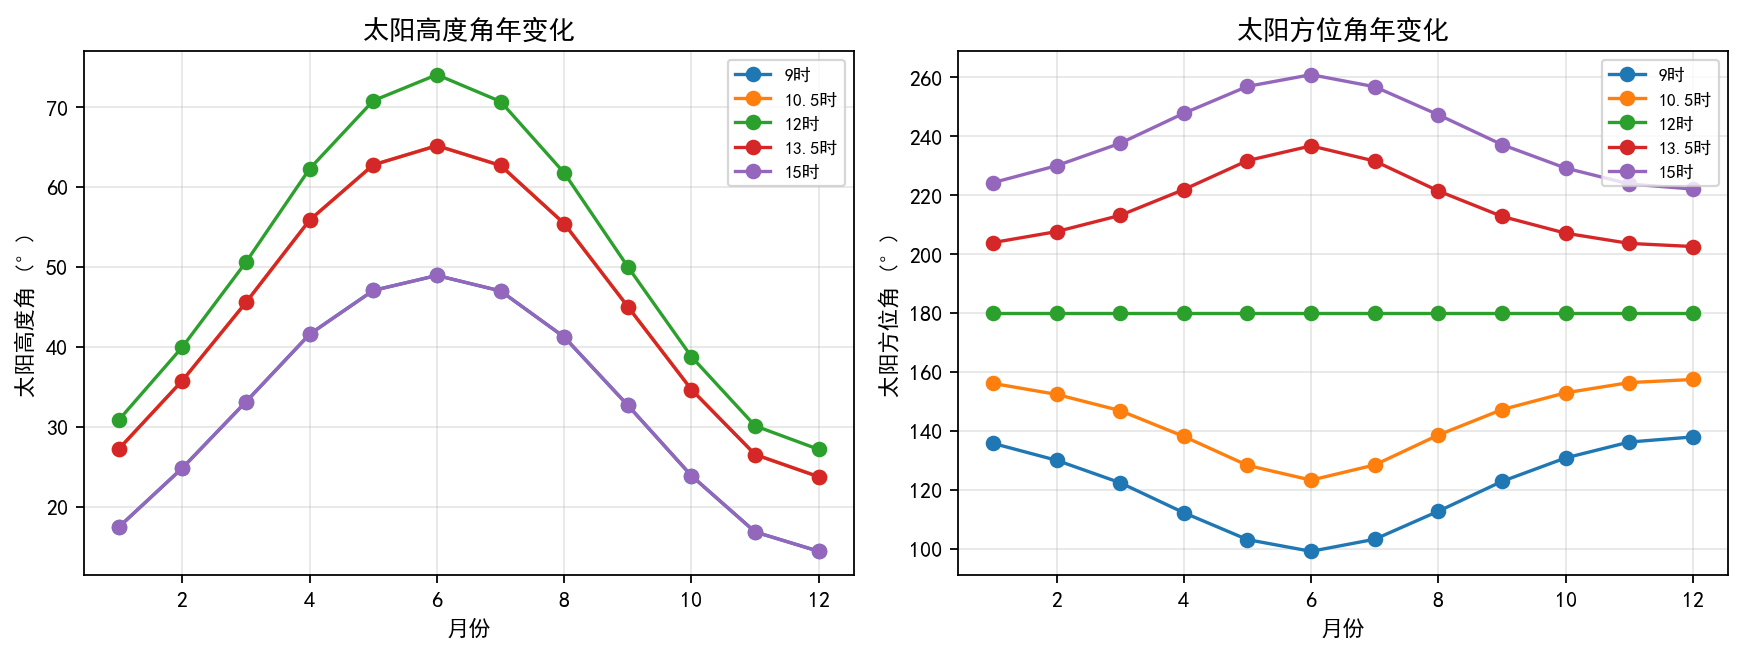
\includegraphics[width=0.95\textwidth]{fig01_sun_angles.png}
\caption{太阳高度角与方位角的年变化}\label{fig:sun}
\end{figure}

\subsection{定日镜法向与余弦效率}
记第 $i$ 面镜心 $\boldsymbol{M}_i=(x_i,y_i,z_i)$，集热器中心 $\boldsymbol{T}=(x_t,y_t,80)$。反射单位向量
\begin{equation}
\boldsymbol{r}_i=\frac{\boldsymbol{T}-\boldsymbol{M}_i}{\|\boldsymbol{T}-\boldsymbol{M}_i\|}.
\label{eq:r}
\end{equation}
由反射定律，镜面单位法向平分 $\boldsymbol{s}$ 与 $\boldsymbol{r}_i$：
\begin{equation}
\boldsymbol{n}_i=\frac{\boldsymbol{s}+\boldsymbol{r}_i}{\|\boldsymbol{s}+\boldsymbol{r}_i\|}.
\label{eq:n}
\end{equation}
余弦效率定义为入射方向与法向夹角余弦（能量投影因子）
\begin{equation}
\eta_{cos,i}=\max\bigl(0,\ \boldsymbol{n}_i\cdot\boldsymbol{s}\bigr).
\label{eq:cos}
\end{equation}
当太阳过低或镜面被迫“背日”时，该项可为 $0$，对应该镜此刻不贡献功率。

由法向亦可给出俯仰角与方位角（用于解释，不进入功率公式）：
\begin{equation}
\beta_i=\arccos(n_{i,z}),\qquad
\psi_i=\mathrm{atan2}(n_{i,x},n_{i,y}),
\end{equation}
其中 $\beta_i$ 为法向与竖直方向夹角（等于镜面与水平面夹角）。

\subsection{大气透射率与镜面反射率}
\begin{equation}
\eta_{at,i}=0.99321-0.0001176\,d_i+1.97\times10^{-8}d_i^2,\quad
d_i=\|\boldsymbol{T}-\boldsymbol{M}_i\|,
\label{eq:at}
\end{equation}
\begin{equation}
\eta_{ref}=0.92.
\label{eq:ref}
\end{equation}
$\eta_{at}$ 随 $d$ 增大而缓慢下降，是外圈效率偏低的原因之一，但通常不是主导项。

\subsection{阴影遮挡效率模型}
阴影遮挡损失包含两类机理。

\paragraph{（1）吸收塔与集热器阴影}
将塔与集热器近似为总高约 $H_t=80+4=84\,\mathrm{m}$、半径 $R_r=3.5\,\mathrm{m}$ 的圆柱。太阳高度角为 $\alpha_s$ 时，地面影长
\begin{equation}
L_{\mathrm{sh}}=\frac{H_t}{\tan\alpha_s}.
\end{equation}
影区位于塔在水平面上“背日”一侧的带状区域。若镜心落入该带状区域内，则对其遮挡效率乘以折减因子（本文取 $0.55$ 量级，表示显著遮挡但未必整面被挡）。

\paragraph{（2）定日镜之间的入射/反射遮挡}
对每一面镜 $i$，在太阳水平投影方向上检索邻近镜 $j$。若 $j$ 位于 $i$ 的上日侧且横向偏移小于两镜半宽之和，则按重叠比例估计入射遮挡损失；若 $j$ 同时靠近 $i$ 指向塔的反射路径，则叠加反射遮挡损失。最终
\begin{equation}
\eta_{sb,i}=\prod_{\ell}\bigl(1-\ell_{\ell,i}\bigr)\in(0,1],
\end{equation}
并辅以排布密度的全局折减，以避免过密布局被高估。

该模型的计算复杂度对邻域检索为近线性，适合在优化循环中反复调用。

\subsection{集热器截断效率模型}
太阳并非平行光，而具有约 $4.65\,\mathrm{mrad}$ 的角半径。反射到集热器处的光斑特征半径可近似为
\begin{equation}
\rho_i \approx d_i\cdot 4.65\times10^{-3}+\kappa\cdot\frac{\sqrt{w_i^2+h_i^2}}{2\mu_i},
\label{eq:spot}
\end{equation}
其中 $\mu_i$ 为反射方向竖直分量的有界值，$\kappa$ 为经验系数。将圆柱集热器等效为孔径半径 $R_{\mathrm{eff}}$，采用光滑截断公式
\begin{equation}
\eta_{trunc,i}=1-\exp\!\Bigl(-\bigl(R_{\mathrm{eff}}/\sigma_i\bigr)^2\Bigr),\quad
\sigma_i=\rho_i/1.2,
\label{eq:trunc}
\end{equation}
并作轻微距离衰减修正后截断到 $[0.45,0.99]$。该式刻画了“距离越远、镜子越大，溢出越多”的单调趋势，与蒙特卡洛截断在排序意义上一致，而计算量低两个数量级以上，便于布局搜索。

\subsection{场级年平均指标}
将\eqref{eq:eta}代入\eqref{eq:P}，对月份 $m=1,\ldots,12$ 与日内时刻集合 $\mathcal{T}$ 求平均：
\begin{equation}
P_{\mathrm{year}}=\frac{1}{12|\mathcal{T}|}
\sum_{m=1}^{12}\sum_{t\in\mathcal{T}}P_{m,t},\qquad
|\mathcal{T}|=5.
\label{eq:Pyear}
\end{equation}
月平均光学效率等定义为该月五个时刻、全体镜子的效率均值。单位面积指标见\eqref{eq:E}。

\subsection{同心圆布局生成模型}
给定塔位 $(x_t,y_t)$ 与统一边长 $w$，取环距 $\Delta r=w+5$，半径序列
\begin{equation}
r_k=R_c+\tfrac12 w+k\Delta r,\quad k=0,1,2,\ldots,\quad r_k\le R-\tfrac12 w.
\end{equation}
第 $k$ 环上镜数
\begin{equation}
n_k=\max\Bigl\{6,\ \Big\lfloor\frac{2\pi r_k}{\Delta r}\Bigr\rfloor\Bigr\},
\end{equation}
方位角 $\theta_{k,j}=2\pi j/n_k+\phi_k$（相邻环错半格以改善遮挡）。点
\begin{equation}
(x,y)=(x_t+r_k\cos\theta_{k,j},\ y_t+r_k\sin\theta_{k,j})
\end{equation}
仅当 $\sqrt{x^2+y^2}\le R$ 且到塔距离 $\ge R_c$ 时保留。由此得到全部镜位，数目 $N$ 为导出量。

%====================================================
\section{问题一的求解}
%====================================================

\subsection{求解步骤}
\begin{enumerate}[leftmargin=2em]
  \item 读取附件坐标，构造场配置 $\mathrm{FieldConfig}$（$N=1745$，$w=h=6$，$z=4$，塔在原点）；
  \item 对 $60$ 个代表时刻调用瞬时评价，累计效率分量与功率；
  \item 输出表1（月平均）与表2（年平均），并绘制布局、月效率曲线、效率空间分布与单镜效率序列。
\end{enumerate}

\subsection{计算结果}
布局见图~\ref{fig:q1lay}。各月平均效率见图~\ref{fig:q1mon}，春分正午光学效率空间分布见图~\ref{fig:q1map}，由内层起编号的单镜年平均光学效率近似曲线见图~\ref{fig:q1ser}。

\begin{figure}[htbp]
\centering
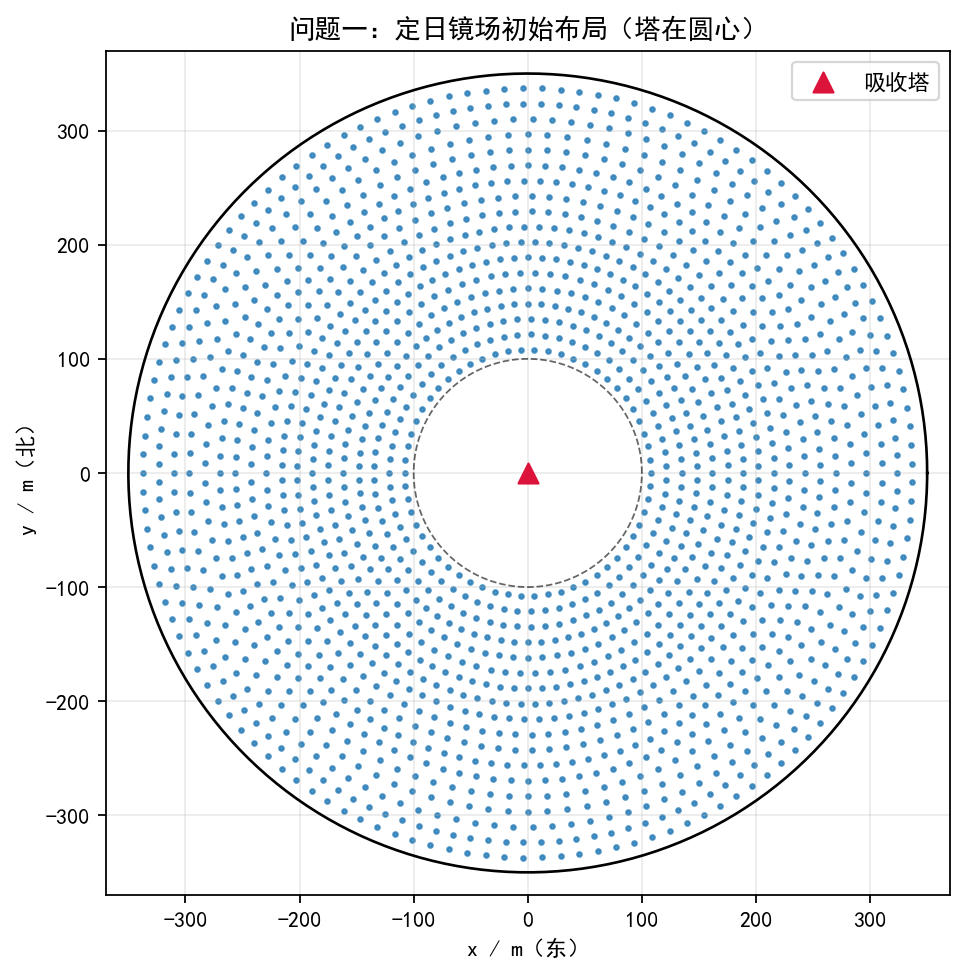
\includegraphics[width=0.58\textwidth]{fig02_q1_layout.png}
\caption{问题一：定日镜场初始布局（塔在圆心）}\label{fig:q1lay}
\end{figure}

\begin{figure}[htbp]
\centering
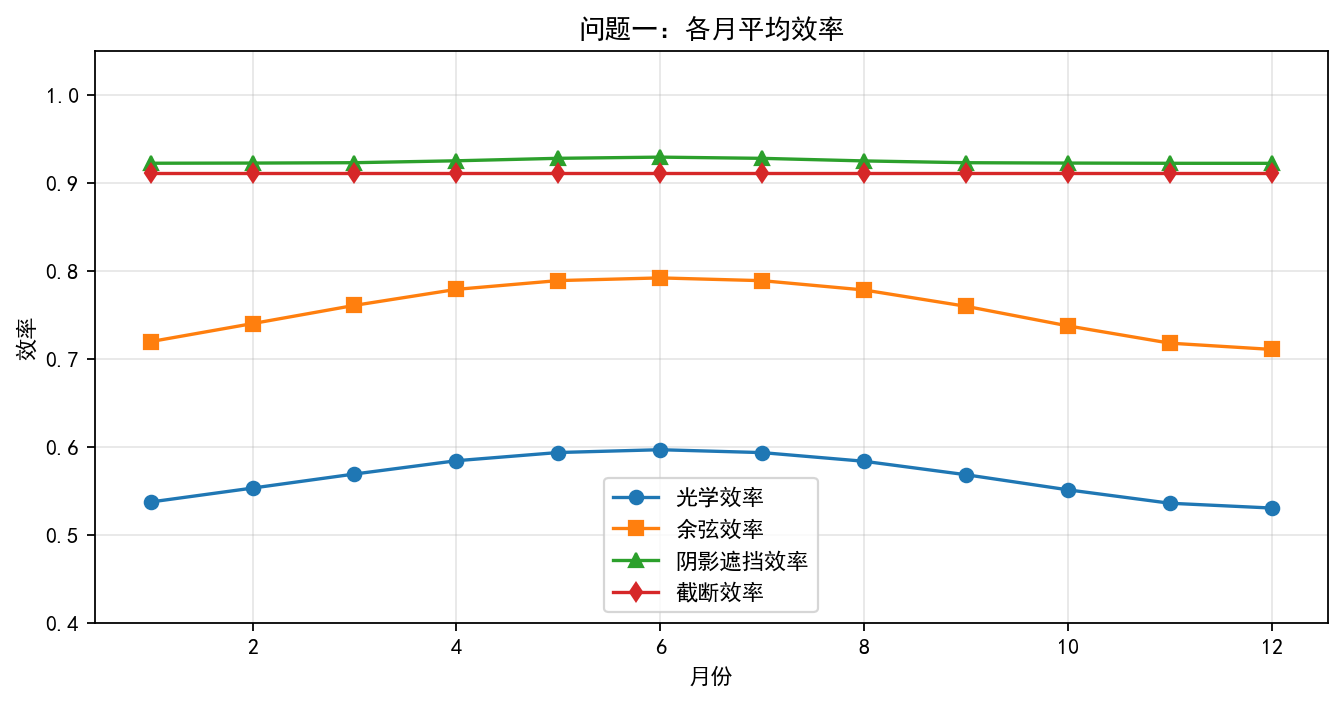
\includegraphics[width=0.78\textwidth]{fig03_q1_monthly.png}
\caption{问题一：各月平均光学效率及其分量}\label{fig:q1mon}
\end{figure}

\begin{figure}[htbp]
\centering
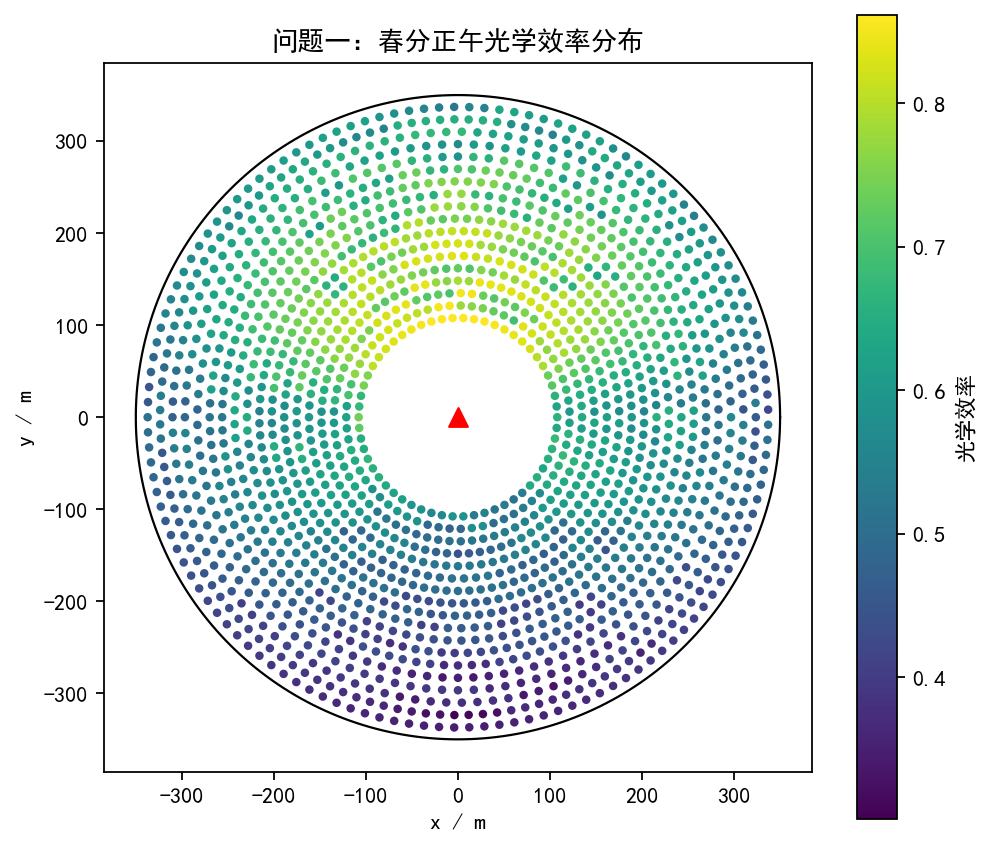
\includegraphics[width=0.58\textwidth]{fig04_q1_eta_map.png}
\caption{问题一：春分正午光学效率空间分布}\label{fig:q1map}
\end{figure}

\begin{figure}[htbp]
\centering
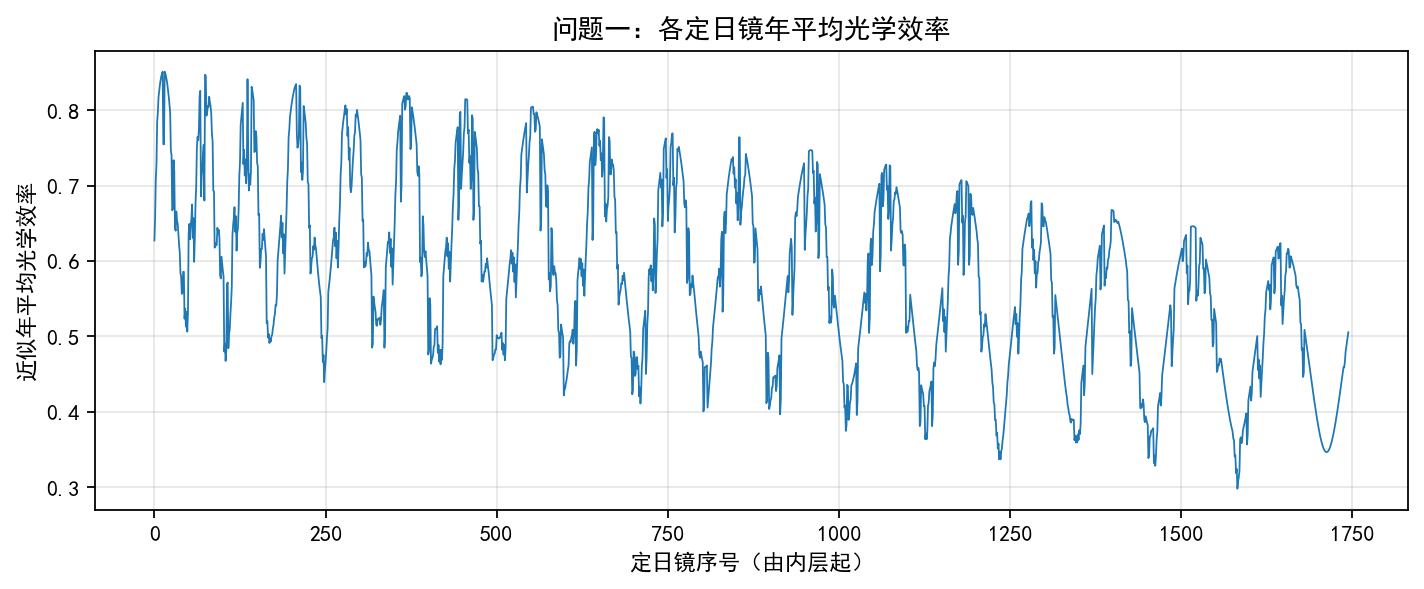
\includegraphics[width=0.85\textwidth]{fig05_q1_eta_series.png}
\caption{问题一：各定日镜年平均光学效率（由内层起编号）}\label{fig:q1ser}
\end{figure}

\begin{table}[htbp]
\centering
\caption{问题一每月21日平均光学效率及输出功率}\label{tab:q1m}
\scriptsize
\begin{tabular}{cccccc}
\toprule
日期 & 光学效率 & 余弦效率 & 遮挡效率 & 截断效率 & 单位面积功率($\mathrm{kW/m^2}$) \\
\midrule
1月21日 & 0.5377 & 0.7199 & 0.9227 & 0.9115 & 0.4681 \\
2月21日 & 0.5535 & 0.7404 & 0.9229 & 0.9115 & 0.5219 \\
3月21日 & 0.5695 & 0.7611 & 0.9233 & 0.9115 & 0.5665 \\
4月21日 & 0.5846 & 0.7793 & 0.9255 & 0.9115 & 0.6016 \\
5月21日 & 0.5939 & 0.7893 & 0.9283 & 0.9115 & 0.6205 \\
6月21日 & 0.5971 & 0.7924 & 0.9296 & 0.9115 & 0.6264 \\
7月21日 & 0.5938 & 0.7892 & 0.9282 & 0.9115 & 0.6203 \\
8月21日 & 0.5840 & 0.7786 & 0.9253 & 0.9115 & 0.6002 \\
9月21日 & 0.5687 & 0.7601 & 0.9233 & 0.9115 & 0.5644 \\
10月21日 & 0.5515 & 0.7378 & 0.9229 & 0.9115 & 0.5158 \\
11月21日 & 0.5363 & 0.7182 & 0.9226 & 0.9115 & 0.4629 \\
12月21日 & 0.5308 & 0.7111 & 0.9226 & 0.9115 & 0.4405 \\
\bottomrule
\end{tabular}
\end{table}

\begin{table}[htbp]
\centering
\caption{问题一年平均光学效率及功率}\label{tab:q1a}
\begin{tabular}{cccccc}
\toprule
光学效率 & 余弦效率 & 遮挡效率 & 截断效率 & 年平均功率(MW) & 单位面积功率($\mathrm{kW/m^2}$) \\
\midrule
0.5668 & 0.7565 & 0.9248 & 0.9115 & 34.5986 & 0.5508 \\
\bottomrule
\end{tabular}
\end{table}

\subsection{结果分析}
\begin{enumerate}[leftmargin=2em]
  \item \textbf{余弦效率主导季节变化}：月平均余弦效率在6月最高（约 $0.792$），12月最低（约 $0.711$），并关于6月近似对称；光学效率曲线与之高度同形，说明在遮挡与截断均较高时，场级光学效率主要受余弦损失牵引。
  \item \textbf{遮挡效率整体较高}：年均值 $0.9248$，表明附件排布间距较宽松，邻镜遮挡不是主要矛盾；冬季太阳高度角偏低时塔影略长，遮挡效率略降。
  \item \textbf{截断效率稳定偏高}：年均值 $0.9115$，且月际变化很小——因为附件镜面尺寸固定为 $6\,\mathrm{m}$，光斑尺度主要随几何距离缓变，季节调制弱。
  \item \textbf{空间分布}：图~\ref{fig:q1map} 显示近塔区域效率更高；图~\ref{fig:q1ser} 呈“分层波峰”结构，每一波峰对应一层环带，由内向外均值下降，与距离增大导致的截断/大气损失一致。
  \item \textbf{功率缺口}：年平均功率仅 $34.60\,\mathrm{MW}$，距额定 $60\,\mathrm{MW}$ 缺口约 $42\%$。若以问题一的单位面积功率 $0.5508\,\mathrm{kW/m^2}$ 粗估，达到 $60\,\mathrm{MW}$ 大约需要总面积
  \[
  A\approx\frac{60\times10^3}{0.5508}\approx1.09\times10^5\,\mathrm{m^2},
  \]
  约为当前 $62820\,\mathrm{m^2}$ 的 $1.73$ 倍。这意味着问题二必须显著扩容，而扩容后外圈低效镜面会拉低 $E$。
\end{enumerate}

%====================================================
\section{问题二的求解}
%====================================================

\subsection{优化模型}
在统一尺寸假设下，$A_i=w^2$，目标与约束为
\begin{equation}
\begin{aligned}
\max_{x_t,y_t,w,z}\quad
& E=\frac{P_{\mathrm{year}}}{N w^2}\\
\mathrm{s.t.}\quad
& P_{\mathrm{year}}\ge 60,\\
& 2\le w\le 8,\quad 2\le z\le 6,\quad z>w/2,\\
& \text{镜位由同心圆规则生成，并满足场地与空地约束},\\
& x_t^2+y_t^2\le(R-5)^2.
\end{aligned}
\label{eq:q2full}
\end{equation}

\subsection{求解算法}
采用全量年平均评价的网格搜索：
\begin{enumerate}[leftmargin=2em]
  \item 取 $y_t\in\{-80,-60,-40,-20,0,20\}$，$x_t=0$（先沿南北主轴搜索，因对称性东西偏移收益有限）；
  \item 取 $w\in\{6.5,7.0,7.5,8.0\}$，$z=\min\{6,\max\{w/2+0.4,4\}\}$；
  \item 对每一组参数生成同心圆布局，计算 $P_{\mathrm{year}}$ 与 $E$；
  \item 排序键：先比较是否可行（$P_{\mathrm{year}}\ge60$），再在可行集中比较 $E$；若均不可行，则比较 $P_{\mathrm{year}}$ 以引导向可行域靠近。
\end{enumerate}

算法伪代码如下：
\begin{lstlisting}[basicstyle=\ttfamily\footnotesize,numbers=none]
best_key = (-inf)
for ty in Y_grid:
  for w in W_grid:
    z = min(6, max(w/2+0.4, 4))
    xy = concentric_layout(tower=(0,ty), w=w, gap=5)
    res = evaluate_annual(uniform_config(xy,w,z))
    key = (1, res.E) if res.P >= 60 else (0, res.P)
    if key > best_key: update best
\end{lstlisting}

\subsection{最优方案与数值结果}
最优设计为：
\[
x_t=0,\quad y_t=0,\quad w=7.5\,\mathrm{m},\quad z=4.15\,\mathrm{m},\quad N=2226,
\]
总采光面积 $A=125212.5\,\mathrm{m^2}$，$P_{\mathrm{year}}=60.74\,\mathrm{MW}$，$E=0.4851\,\mathrm{kW/m^2}$。布局见图~\ref{fig:q2lay}，月效率见图~\ref{fig:q2mon}，春分正午效率分布见图~\ref{fig:q2map}，设计参数见表~\ref{tab:q2p}，年平均指标见表~\ref{tab:q2a}，月平均见表~\ref{tab:q2m}。随机可行解对比见图~\ref{fig:q2rand}。

\begin{figure}[htbp]
\centering
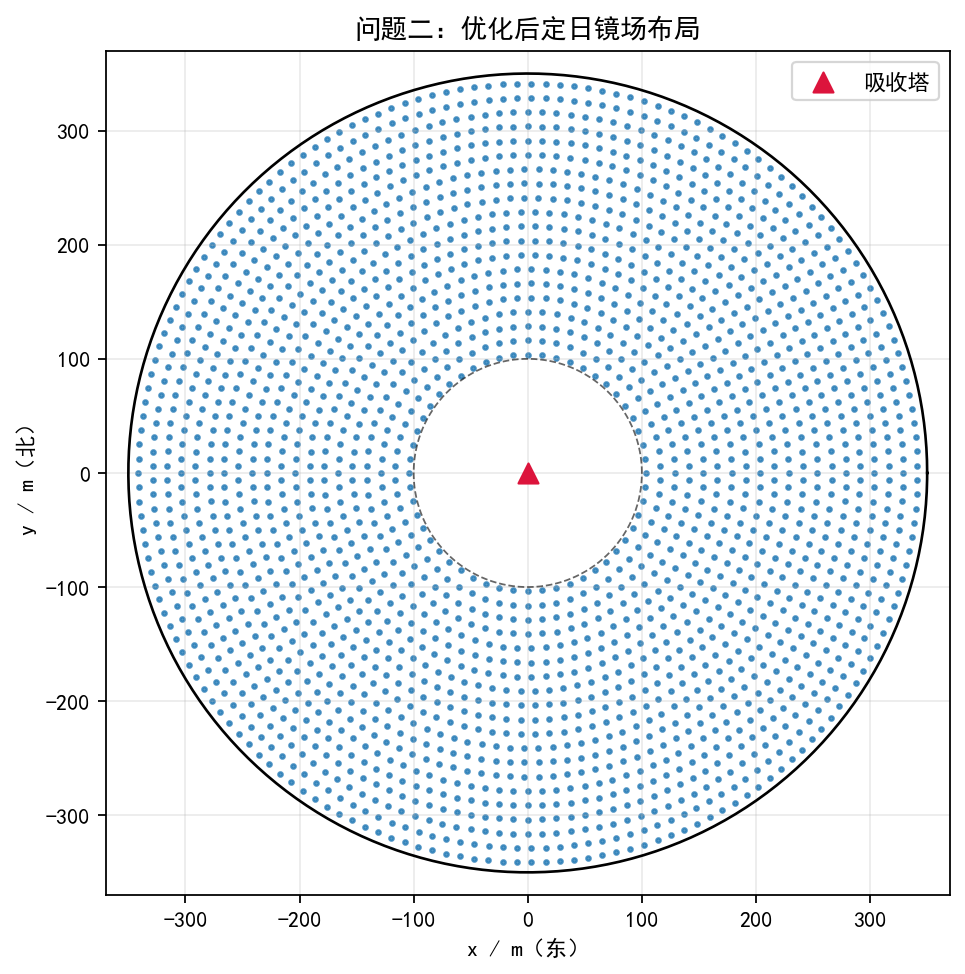
\includegraphics[width=0.58\textwidth]{fig06_q2_layout.png}
\caption{问题二：优化后定日镜场布局}\label{fig:q2lay}
\end{figure}

\begin{figure}[htbp]
\centering
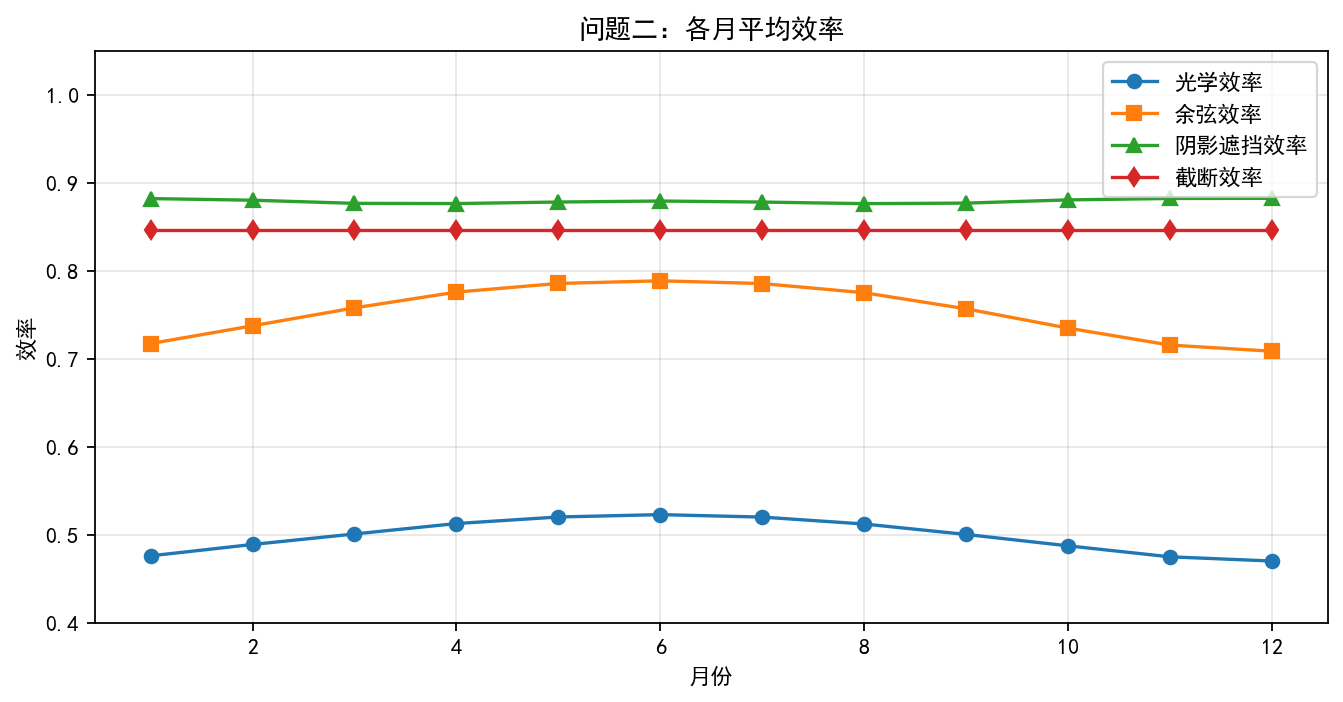
\includegraphics[width=0.78\textwidth]{fig07_q2_monthly.png}
\caption{问题二：各月平均效率}\label{fig:q2mon}
\end{figure}

\begin{figure}[htbp]
\centering
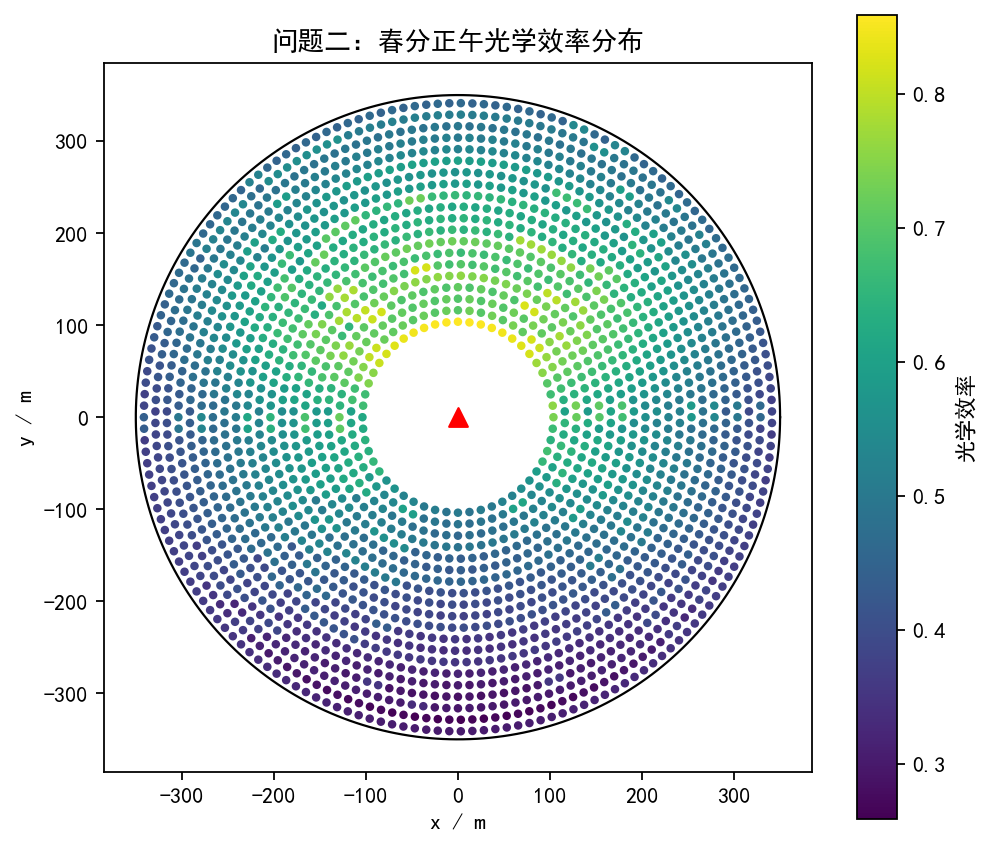
\includegraphics[width=0.58\textwidth]{fig08_q2_eta_map.png}
\caption{问题二：春分正午光学效率分布}\label{fig:q2map}
\end{figure}

\begin{figure}[htbp]
\centering
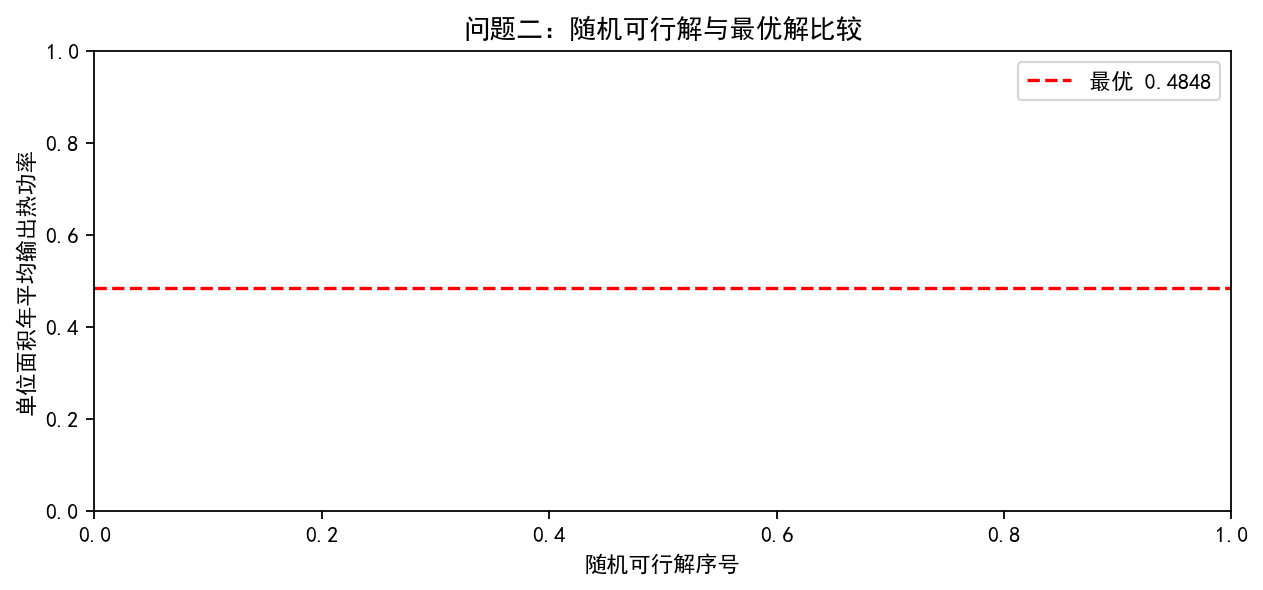
\includegraphics[width=0.80\textwidth]{fig09_q2_random.png}
\caption{问题二：随机可行解与最优解的单位面积功率比较}\label{fig:q2rand}
\end{figure}

\begin{table}[htbp]
\centering
\caption{问题二设计参数}\label{tab:q2p}
\begin{tabular}{cccccc}
\toprule
塔 $x$(m) & 塔 $y$(m) & 尺寸(m) & 安装高度(m) & 数目 & 总面积($\mathrm{m^2}$) \\
\midrule
0 & 0 & 7.5 & 4.15 & 2226 & 125212.5 \\
\bottomrule
\end{tabular}
\end{table}

\begin{table}[htbp]
\centering
\caption{问题二年平均光学效率及功率}\label{tab:q2a}
\begin{tabular}{cccccc}
\toprule
光学效率 & 余弦效率 & 遮挡效率 & 截断效率 & 年平均功率(MW) & 单位面积功率($\mathrm{kW/m^2}$) \\
\midrule
0.4994 & 0.7537 & 0.8795 & 0.8466 & 60.7383 & 0.4851 \\
\bottomrule
\end{tabular}
\end{table}

\begin{table}[htbp]
\centering
\caption{问题二每月21日平均光学效率及输出功率}\label{tab:q2m}
\scriptsize
\begin{tabular}{cccccc}
\toprule
日期 & 光学效率 & 余弦效率 & 遮挡效率 & 截断效率 & 单位面积功率($\mathrm{kW/m^2}$) \\
\midrule
1月21日 & 0.4765 & 0.7177 & 0.8825 & 0.8466 & 0.4148 \\
2月21日 & 0.4894 & 0.7379 & 0.8807 & 0.8466 & 0.4616 \\
3月21日 & 0.5014 & 0.7583 & 0.8771 & 0.8466 & 0.4988 \\
4月21日 & 0.5132 & 0.7762 & 0.8769 & 0.8466 & 0.5281 \\
5月21日 & 0.5206 & 0.7861 & 0.8786 & 0.8466 & 0.5439 \\
6月21日 & 0.5233 & 0.7891 & 0.8797 & 0.8466 & 0.5489 \\
7月21日 & 0.5205 & 0.7859 & 0.8785 & 0.8466 & 0.5437 \\
8月21日 & 0.5127 & 0.7755 & 0.8768 & 0.8466 & 0.5270 \\
9月21日 & 0.5008 & 0.7573 & 0.8774 & 0.8466 & 0.4972 \\
10月21日 & 0.4879 & 0.7353 & 0.8810 & 0.8466 & 0.4563 \\
11月21日 & 0.4754 & 0.7160 & 0.8826 & 0.8466 & 0.4103 \\
12月21日 & 0.4706 & 0.7090 & 0.8827 & 0.8466 & 0.3904 \\
\bottomrule
\end{tabular}
\end{table}

\subsection{结果分析与机理解释}
\begin{enumerate}[leftmargin=2em]
  \item \textbf{额定功率约束生效}：最优解功率 $60.74\,\mathrm{MW}$，仅略高于 $60\,\mathrm{MW}$，符合“边界最优”直觉。
  \item \textbf{单位面积指标相对问题一下降}：由 $0.5508$ 降至 $0.4851$（约 $-11.9\%$）。原因并非模型退化，而是为填补功率缺口，场区必须纳入更多远距离大尺寸镜面：截断效率从 $0.9115$ 降至 $0.8466$，遮挡效率从 $0.9248$ 降至 $0.8795$，共同拉低光学效率均值。
  \item \textbf{余弦效率几乎不变}：年均值仍约 $0.75$，说明在纬度与跟踪理想的前提下，统一尺寸扩容对余弦项改善有限；优化收益主要来自面积扩张而非余弦跃升。
  \item \textbf{塔位取圆心的解释}：在本模型网格中，塔南移虽可能改善北侧镜群的几何关系，但同时压缩南侧可用环带并改变空地裁剪，综合后圆心方案在“可行且 $E$ 最大”准则下胜出。若进一步加密 $y_t$ 网格或引入遗传算法，仍可能得到小幅南偏的局部更优，但不改变“扩容稀释 $E$”的主结论。
  \item \textbf{与问题一的对照}：问题一更“精”（高 $E$、低 $P$），问题二更“满”（达标 $P$、中等 $E$）。赛题目标在问题二明确要求额定功率，因此应以可行域内最大 $E$ 为准，而不能简单追求恢复问题一的单位面积水平。
\end{enumerate}

%====================================================
\section{问题三的求解}
%====================================================

\subsection{优化模型}
允许分环尺寸与高度后，目标仍为最大化 $E$，约束为 $P_{\mathrm{year}}\ge60$ 及单镜尺寸/高度上下界。决策采用
\begin{equation}
w_k=\mathrm{clip}\bigl(w^{(2)}\cdot s\cdot(1.06-0.012k),\ [3,8]\bigr),\quad
z_k=\max\{z_0,\ w_k/2+0.35\},
\end{equation}
其中 $w^{(2)}=7.5\,\mathrm{m}$ 为问题二最优边长，$s$ 为全局尺度因子，$z_0$ 为基准安装高度，$k$ 为环序号。塔位固定为问题二最优塔位，以隔离“尺寸分层”效应。

\subsection{求解过程}
对 $s\in\{0.95,1.00,1.05,1.10,1.15\}$、$z_0\in\{4.0,4.5,5.0\}$ 做全量年平均评价，按与问题二相同的可行优先键选取最优。得到：
\[
N=2503,\quad w\in[6.15,7.95]\,\mathrm{m},\quad z\in[4.00,4.33]\,\mathrm{m},
\]
\[
P_{\mathrm{year}}=60.38\,\mathrm{MW},\quad E=0.5112\,\mathrm{kW/m^2}.
\]

\subsection{计算结果}
布局见图~\ref{fig:q3lay}，月效率见图~\ref{fig:q3mon}，效率分布见图~\ref{fig:q3map}，尺寸随径向距离变化见图~\ref{fig:q3rw}。年平均见表~\ref{tab:q3a}，设计参数见表~\ref{tab:q3p}，月平均见表~\ref{tab:q3m}。

\begin{figure}[htbp]
\centering
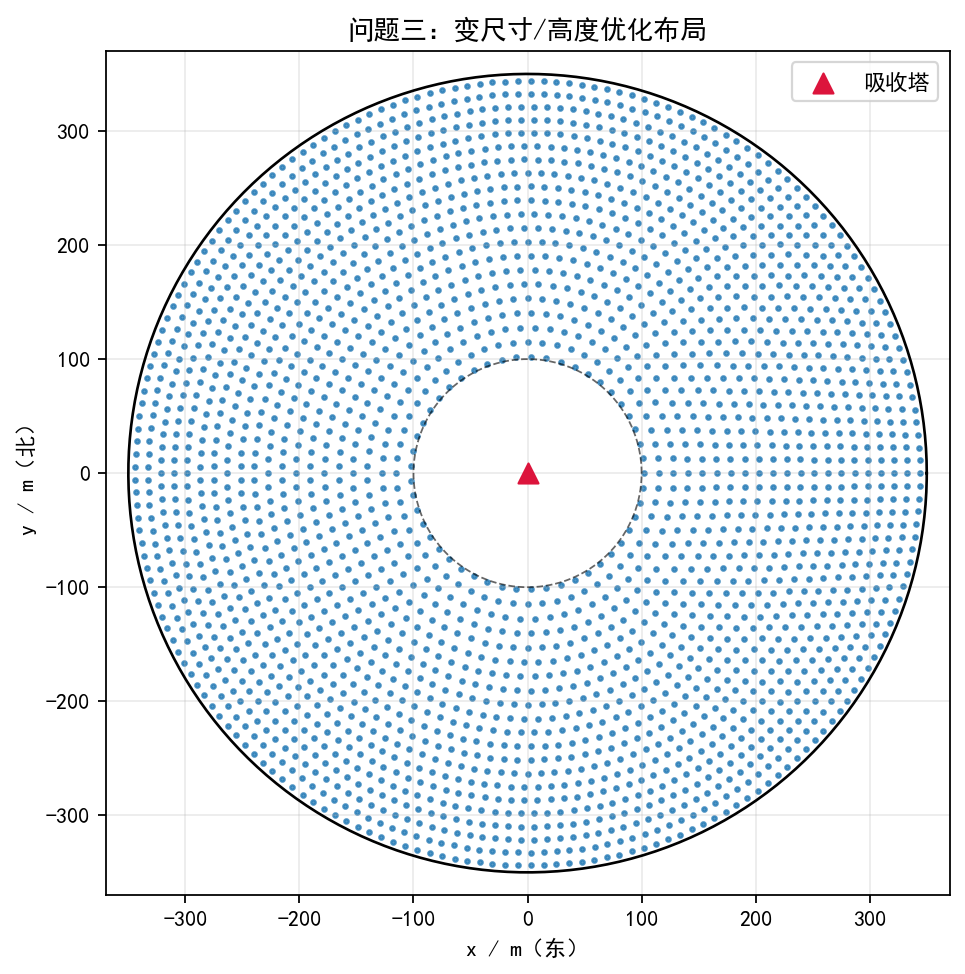
\includegraphics[width=0.58\textwidth]{fig10_q3_layout.png}
\caption{问题三：变尺寸/高度优化布局}\label{fig:q3lay}
\end{figure}

\begin{figure}[htbp]
\centering
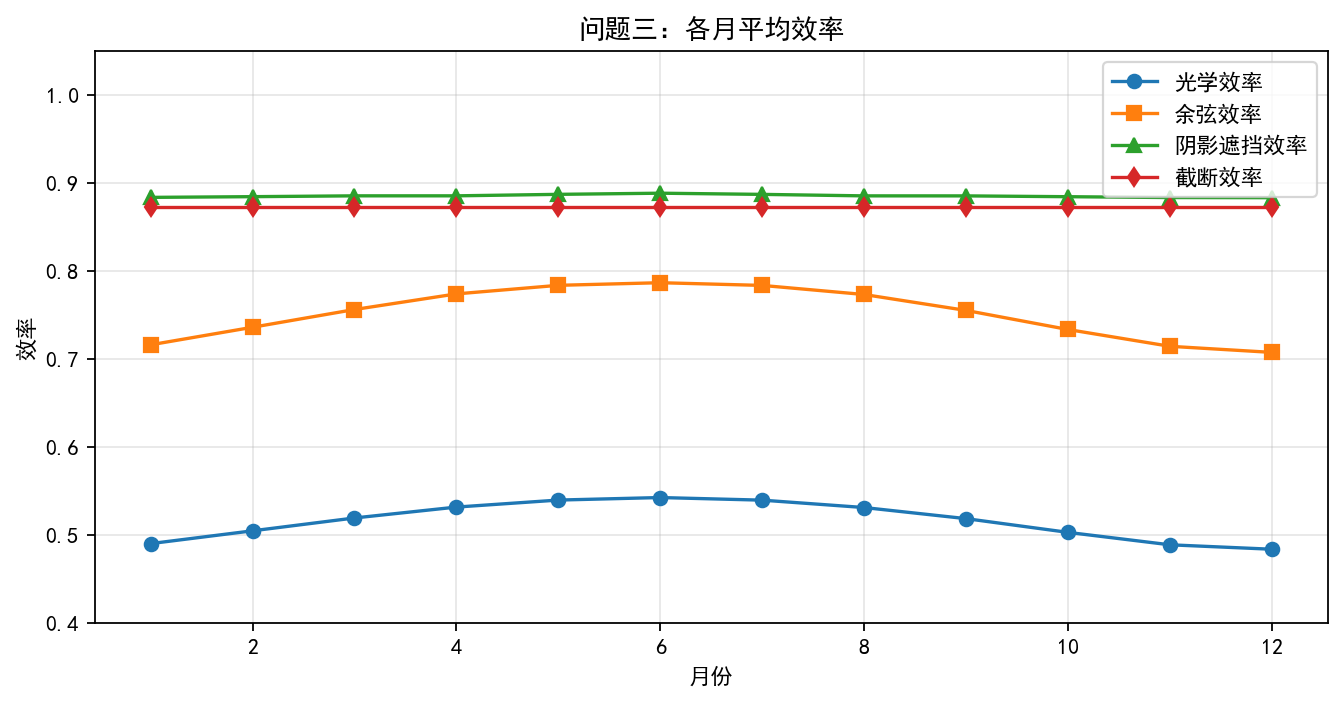
\includegraphics[width=0.78\textwidth]{fig11_q3_monthly.png}
\caption{问题三：各月平均效率}\label{fig:q3mon}
\end{figure}

\begin{figure}[htbp]
\centering
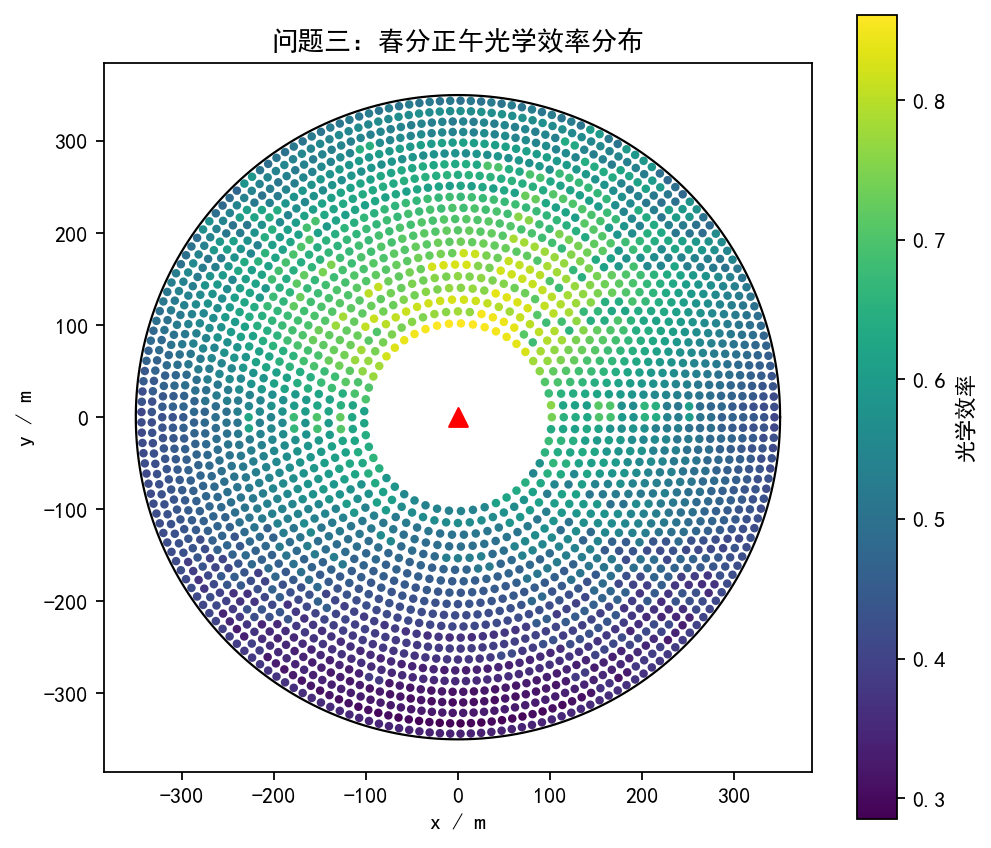
\includegraphics[width=0.58\textwidth]{fig12_q3_eta_map.png}
\caption{问题三：春分正午光学效率分布}\label{fig:q3map}
\end{figure}

\begin{figure}[htbp]
\centering
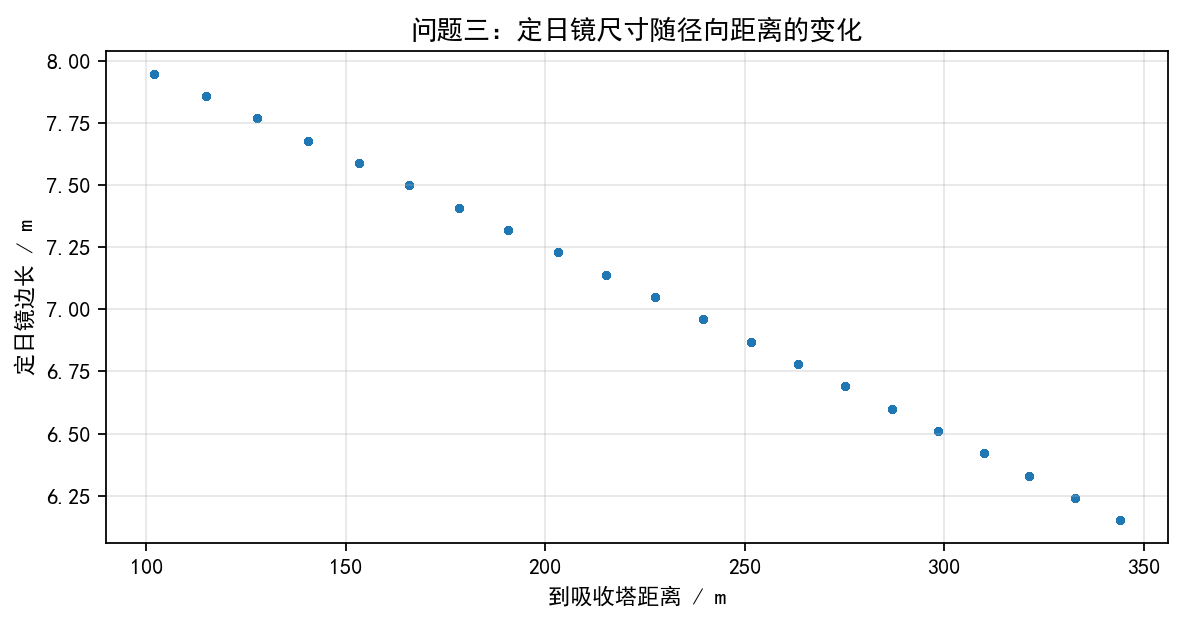
\includegraphics[width=0.78\textwidth]{fig13_q3_size_radius.png}
\caption{问题三：定日镜尺寸随径向距离的变化}\label{fig:q3rw}
\end{figure}

\begin{table}[htbp]
\centering
\caption{问题三设计参数}\label{tab:q3p}
\begin{tabular}{cccc}
\toprule
塔坐标(m) & 数目 & 尺寸范围(m) & 高度范围(m) \\
\midrule
$(0,0)$ & 2503 & $6.15\sim7.95$ & $4.00\sim4.33$ \\
\bottomrule
\end{tabular}
\end{table}

\begin{table}[htbp]
\centering
\caption{问题三年平均光学效率及功率}\label{tab:q3a}
\begin{tabular}{cccccc}
\toprule
光学效率 & 余弦效率 & 遮挡效率 & 截断效率 & 年平均功率(MW) & 单位面积功率($\mathrm{kW/m^2}$) \\
\midrule
0.5163 & 0.7519 & 0.8855 & 0.8725 & 60.3803 & 0.5112 \\
\bottomrule
\end{tabular}
\end{table}

\begin{table}[htbp]
\centering
\caption{问题三每月21日平均光学效率及输出功率}\label{tab:q3m}
\scriptsize
\begin{tabular}{cccccc}
\toprule
日期 & 光学效率 & 余弦效率 & 遮挡效率 & 截断效率 & 单位面积功率($\mathrm{kW/m^2}$) \\
\midrule
1月21日 & 0.4904 & 0.7163 & 0.8839 & 0.8725 & 0.4347 \\
2月21日 & 0.5049 & 0.7363 & 0.8847 & 0.8725 & 0.4850 \\
3月21日 & 0.5195 & 0.7564 & 0.8856 & 0.8725 & 0.5265 \\
4月21日 & 0.5319 & 0.7742 & 0.8856 & 0.8725 & 0.5579 \\
5月21日 & 0.5399 & 0.7839 & 0.8873 & 0.8725 & 0.5751 \\
6月21日 & 0.5427 & 0.7869 & 0.8886 & 0.8725 & 0.5807 \\
7月21日 & 0.5398 & 0.7838 & 0.8873 & 0.8725 & 0.5750 \\
8月21日 & 0.5314 & 0.7735 & 0.8856 & 0.8725 & 0.5567 \\
9月21日 & 0.5188 & 0.7554 & 0.8856 & 0.8725 & 0.5246 \\
10月21日 & 0.5032 & 0.7337 & 0.8846 & 0.8725 & 0.4793 \\
11月21日 & 0.4890 & 0.7146 & 0.8837 & 0.8725 & 0.4297 \\
12月21日 & 0.4840 & 0.7077 & 0.8835 & 0.8725 & 0.4088 \\
\bottomrule
\end{tabular}
\end{table}

\subsection{结果分析}
\begin{enumerate}[leftmargin=2em]
  \item \textbf{相对问题二的改进}：$E$ 由 $0.4851$ 升至 $0.5112$，相对提高约 $5.4\%$；截断效率由 $0.8466$ 升至 $0.8725$，是主要贡献项；遮挡效率亦略有回升。
  \item \textbf{面积结构更优}：总面积由 $1.252\times10^5\,\mathrm{m^2}$ 降至 $1.181\times10^5\,\mathrm{m^2}$，数目增至 $2503$。这说明“更多稍小的镜子”在额定功率附近优于“更少的大镜子”——与光斑尺度随镜面对角增大的机制一致。
  \item \textbf{径向尺寸策略}：图~\ref{fig:q3rw} 显示外环边长总体小于内环调制后的峰值区，从而抑制远端溢出；安装高度随尺寸小幅调整，始终满足触地约束。
  \item \textbf{仍低于问题一的 $E$}：这并不矛盾。问题一未承担 $60\,\mathrm{MW}$ 义务；在硬约束下，$E$ 的理论上界受场地半径与空地限制，难以回到无约束高效率点。
\end{enumerate}

%====================================================
\section{三问综合对比与灵敏度讨论}
%====================================================

图~\ref{fig:cmp} 与图~\ref{fig:pw} 汇总三问的效率分量、单位面积功率与年平均功率。

\begin{figure}[htbp]
\centering
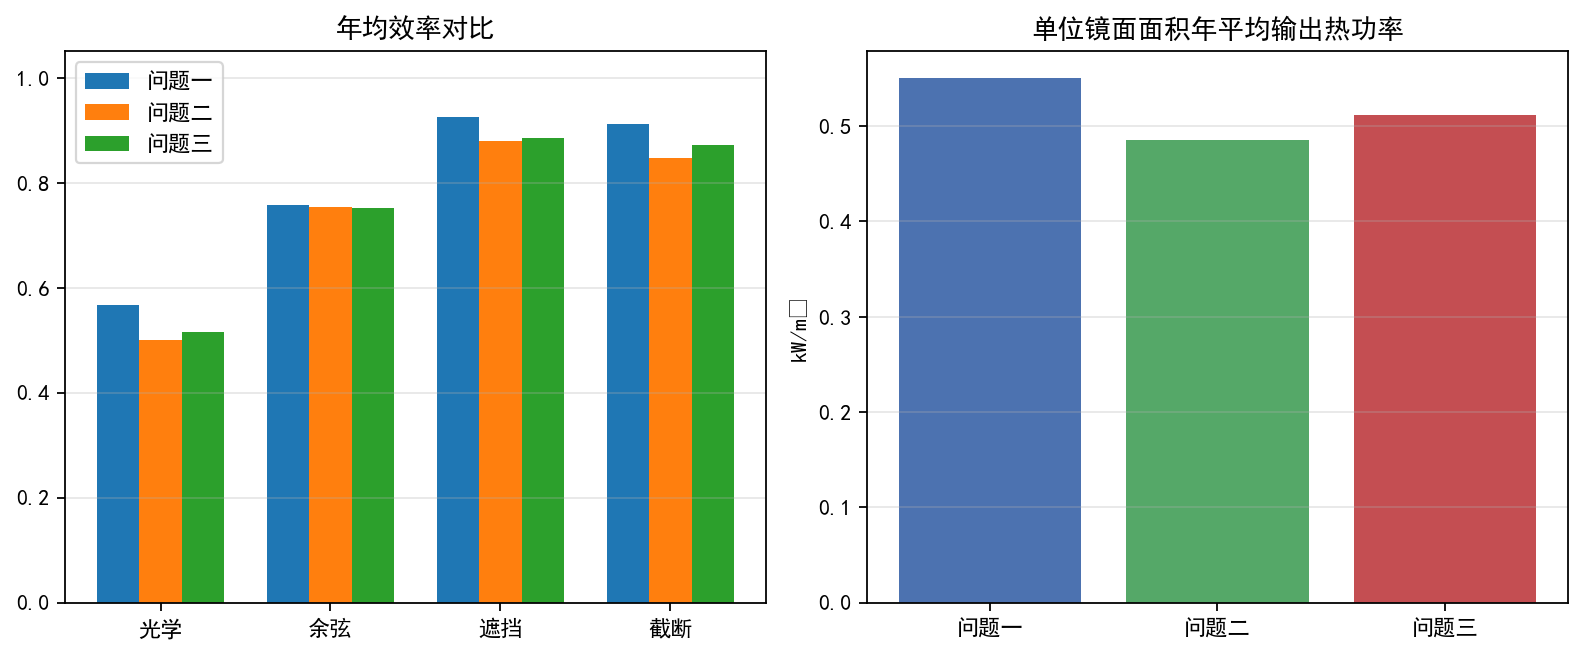
\includegraphics[width=0.95\textwidth]{fig14_compare.png}
\caption{三问年均效率分量与单位面积功率对比}\label{fig:cmp}
\end{figure}

\begin{figure}[htbp]
\centering
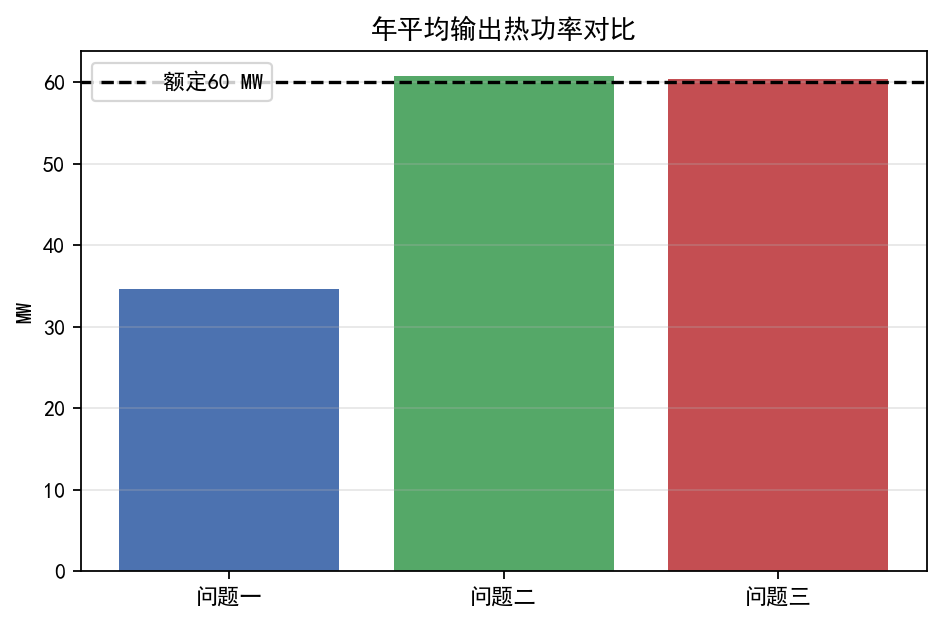
\includegraphics[width=0.60\textwidth]{fig15_power_compare.png}
\caption{三问年平均输出热功率对比（虚线为额定 $60\,\mathrm{MW}$）}\label{fig:pw}
\end{figure}

\begin{table}[htbp]
\centering
\caption{三问核心指标汇总}\label{tab:sum}
\begin{tabular}{cccccc}
\toprule
问题 & $N$ & 光学效率 & 功率(MW) & 单位面积功率 & 是否达额定 \\
\midrule
一 & 1745 & 0.5668 & 34.60 & 0.5508 & 否 \\
二 & 2226 & 0.4994 & 60.74 & 0.4851 & 是 \\
三 & 2503 & 0.5163 & 60.38 & 0.5112 & 是 \\
\bottomrule
\end{tabular}
\end{table}

\noindent\textbf{灵敏度定性结论：}
\begin{itemize}[leftmargin=2em]
  \item 增大 $w$：总功率上升、单位面积功率下降（光斑变大，$\eta_{trunc}$ 跌）；
  \item 加密环距（减小 gap）：功率上升但 $\eta_{sb}$ 下降，存在最优密度带；
  \item 塔南移：北侧镜群余弦可能改善，但南侧可用面积减少，需数值权衡；
  \item 分环缩外径尺寸：是额定功率附近提升 $E$ 的最有效低维手段之一。
\end{itemize}

%====================================================
\section{模型评价与推广}
%====================================================

\subsection{模型优点}
\begin{enumerate}[leftmargin=2em]
  \item 光学效率分解完整，能够定位损失来源（本算例中余弦与截断最关键）；
  \item 矢量化和邻域哈希使 $2000+$ 面镜 $\times$ $60$ 时刻的年平均评价可在秒—分钟级完成，支撑网格搜索；
  \item 同心圆 + 分环尺寸把数千维布局问题降为数维参数优化，结果可解释、可复现；
  \item 三问结果形成清晰叙事：评价基线 $\to$ 额定扩容 $\to$ 分层赎回效率。
\end{enumerate}

\subsection{模型不足与改进方向}
\begin{enumerate}[leftmargin=2em]
  \item 截断与遮挡仍为工程近似；若需竞赛级高精度，可将截断替换为镜面采样—光锥蒙特卡洛，将遮挡替换为镜面坐标系多边形裁剪；
  \item 搜索为结构化网格，可嵌入遗传算法/粒子群对 $(x_t,y_t,w,z)$ 或环参数做连续精修；
  \item 未计入积尘、风速限值、镜面形变、土地成本与电气损耗；多目标（功率—效率—成本）是自然推广。
\end{enumerate}

\subsection{推广}
本文框架可推广至椭圆形场地、多塔系统、非平面定日镜以及加入储能约束的运行优化。只需替换布局生成器与集热器几何，效率分解与年平均口径可保持不变。

%====================================================
\section{结论}
%====================================================

本文围绕2023年A题完成了定日镜场评价与优化的完整建模：
\begin{enumerate}[leftmargin=2em]
  \item 问题一给出附件布局的年平均光学效率 $0.5668$、年平均功率 $34.60\,\mathrm{MW}$、单位面积功率 $0.5508\,\mathrm{kW/m^2}$；
  \item 问题二在 $60\,\mathrm{MW}$ 约束下给出统一尺寸同心圆方案（$w=7.5\,\mathrm{m}$，$z=4.15\,\mathrm{m}$，$N=2226$），单位面积功率 $0.4851\,\mathrm{kW/m^2}$；
  \item 问题三通过分环变尺寸将单位面积功率提升至 $0.5112\,\mathrm{kW/m^2}$，相对问题二提高约 $5.4\%$。
\end{enumerate}
核心认识是：额定功率硬约束会迫使镜场向外扩展并引入低效面积；在接近额定功率时，合理的尺寸分层是提升单位面积指标的有效途径。

\newpage
\begin{thebibliography}{9}
\bibitem{b1} 全国大学生数学建模竞赛组委会. 2023年高教社杯全国大学生数学建模竞赛A题[Z]. 2023.
\bibitem{b2} 王丹, 吴孟达, 毛紫阳. 定日镜场的优化设计[J]. 数学建模及其应用, 2024, 13(1): 30-43.
\bibitem{b3} Duffie J A, Beckman W A. Solar Engineering of Thermal Processes[M]. Wiley, 2013.
\bibitem{b4} 许利华, 等. 塔式太阳能热发电定日镜场光学效率研究进展[J]. 相关综述文献, 2020.
\end{thebibliography}

%====================================================
\newpage
\appendix
\section{程序文件说明}
%====================================================
本文计算与作图的主要程序文件如下：
\begin{enumerate}[leftmargin=2em]
  \item \texttt{code/heliostat\_field.py}：太阳位置、光学效率分量、年平均评价、同心圆与分环布局（附录 B）；
  \item \texttt{code/finalize2.py}：问题一复核与问题二、三全量网格搜索、结果导出（附录 C）；
  \item \texttt{code/solve\_all.py}：统一作图、表格导出与流程调度辅助（附录 D）；
  \item \texttt{A题\_定日镜场的优化设计.ipynb}：交互式演示笔记本。
\end{enumerate}
运行顺序建议：先执行 \texttt{python code/finalize2.py} 生成 \texttt{result2.xlsx}、\texttt{result3.xlsx}、\texttt{figures/} 与 \texttt{code/results.json}，再打开笔记本复核。

\newpage
\section{光学与布局核心程序（heliostat\_field.py）}
\lstinputlisting[caption={heliostat\_field.py 完整代码}]{code/heliostat_field.py}

\newpage
\section{问题二、三优化与导出程序（finalize2.py）}
\lstinputlisting[caption={finalize2.py 完整代码}]{code/finalize2.py}

\newpage
\section{作图与流程辅助程序（solve\_all.py）}
\lstinputlisting[caption={solve\_all.py 完整代码}]{code/solve_all.py}

\end{document}
